%--------------------
% Packages
% -------------------
\documentclass[11pt,a4paper,twocolumn]{article}
\usepackage[utf8x]{inputenc}
% \usepackage[T1]{fontenc}
% \usepackage{mathptmx} % Use Times Font
%\usepackage{gentium}
\usepackage{fontspec}
\setmainfont{Times New Roman}
\usepackage{amsmath} % mathy stuff


\usepackage{graphicx} % Required for including pictures
\usepackage[english]{babel} 
\usepackage[linkcolor=black,pdfborder={0 0 0}]{hyperref} % Format links for pdf
\usepackage{calc} % To reset the counter in the document after title page
\usepackage{enumerate} % Includes lists


\frenchspacing % No double spacing between sentences
\linespread{1.5} % Set linespace
\usepackage[a4paper, lmargin=0.1\paperwidth, rmargin=0.1\paperwidth, tmargin=0.1\paperheight, bmargin=0.1\paperheight]{geometry} %margins
\usepackage{parskip}

 
\usepackage{lipsum} % Used for inserting dummy 'Lorem ipsum' text into the template

%-----------------------
% SET DOCUMENT SPECIFIC DATA
%-----------------------
\newcommand\ModuleCode{ECO00037I}
\newcommand\DocumentTitle{Problem Set 3}
\newcommand\DueDate{November 7, 2023}


%-----------------------
% Set pdf information and add title, fill in the fields
%-----------------------
\hypersetup{
    pdfsubject = {\ModuleCode},
    pdftitle = {\DocumentTitle},
    pdfauthor = {REDACTED},
}

% Graph Stuff: 
\usepackage{pgfplots}
\pgfplotsset{width=0.8\textwidth,compat=1.9}
% We will externalize the figures
\usepgfplotslibrary{external}
\tikzexternalize


%-----------------------
% Header and footer information 
% Use LE / RO for twosided docs 
% https://tex.stackexchange.com/questions/69100/distinguish-even-odd-pages-in-header-with-oneside-option
%-----------------------


\usepackage{fancyhdr}
\renewcommand{\sectionmark}[1]{\markright{#1}{} }
\renewcommand{\subsectionmark}[1]{\markright{\thesubsection\ #1}}
\fancyhead{}
\fancyhead[L]{\DocumentTitle}
\fancyhead[R]{\rightmark}
\fancyfoot{}
\fancyfoot[L]{\ModuleCode}
\fancyfoot[C]{University of York}
\fancyfoot[R]{\thepage}



%-----------------------
% Begin document
%-----------------------
\begin{document} 

\pagestyle{fancy}

\begin{titlepage}
    \begin{center}
        \vspace*{1cm}

        \Huge
        \textbf{\DocumentTitle}

        \Large
        \vspace{0.5cm}
        Microeconomics \ModuleCode

        \vspace{1.5cm}

        \textbf{}

        \vfill

        \vspace{0.8cm}
     
        
\includegraphics[width=0.4\textwidth]{imgs/uoy-logo.png}
            
        Isaac Beight-Welland\\
        University of York\\
        United Kingdom\\
        \DueDate\\
            
    \end{center}
\end{titlepage}



\newpage

\twocolumn[\section*{Problem 3.1}]
\sectionmark{Problem 3.1}

\begin{enumerate}[(a)]

    \item 
    
        The marginal product of labour and capital for the given production function $f(K,L) = K^{\frac{1}{2}}L^{\frac{1}{2}}$ is given respectively by: 
        $$
            \frac{\partial L}{\partial L}=  \frac{K^{\frac{1}{2}}}{2L^{\frac{1}{2}}} = \sqrt{\frac{K}{L}} \qquad \frac{\partial f}{\partial K}=\sqrt{\frac{L}{K}} 
        $$
        The marginal rate of substitution is the rate of change of capital with respect to labour: 
        $$
            MRS = \frac{\partial K}{\partial L} = \frac{\partial K}{\partial f} \div \frac{\partial L}{\partial f} 
        $$
        For PaperInc, the technical rate of substitution is given by:
        $$
            - \sqrt{\frac{L}{K}} \div \sqrt{\frac{K}{L}} = - \sqrt{\frac{L}{K}} \times \sqrt{\frac{L}{K}} = - \frac{L}{K}
        $$
    
    
    \item 
    
        To find the optimal bundle for a 10 units of output we must minimise cost subject to the production function: 
        $$
            \min_{c} \ c = 4K + L \quad \textnormal{s.t} \quad 10 = \sqrt{KL}
        $$
        Rearranging the constraint function for capital and labour: 
        \begin{align*}
            100 &= KL  \\
            L &= 100K^{-1}
        \end{align*}
        Substitute into the cost function: 
        $$
            c= 4K + 100K^{-1}
        $$
        Cost minimised when the marginal output of capital is zero: 
        \begin{gather*}
            \frac{dc}{dK}=4-100K^{-2}=0\\
            4=\frac{100}{K^2}\\
            K=5
        \end{gather*}
        Substitute back into constraint function for labour: 
        \begin{align*}
            10=&\sqrt{5L}\\
            L=&20
        \end{align*}
    
    \item 
    
    The graph below shows the optimal bundle for PaperInc's input costs at the production of 10 output.
    
    \begin{figure}[htbp!]
    \hspace*{2em}
        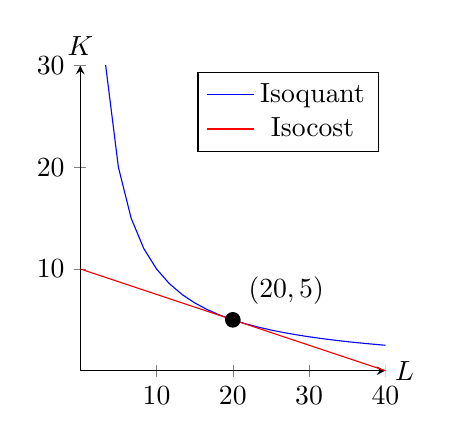
\begin{tikzpicture}
            \begin{axis}[
                axis lines=middle,
                height=0.45\textwidth,
                width=0.45\textwidth,
                ymin=0, ymax=30,
                xmin=0, xmax=40,
                x label style={at={(axis description cs:1,0)},anchor=west},
                y label style={at={(axis description cs:0,1)},rotate=0,anchor=south},
                xlabel={$L$},
                ylabel={$K$}]
                
                \addplot+[domain=0:40, mark size=0]
                    {100/x};
                \addlegendentry{Isoquant}
    
                \addplot+[domain=0:40, mark size=0]
                    {10-0.25*x};
                \addlegendentry{Isocost}
    
                \node[label={45:{$(20,5)$}}, circle, fill, inner sep=2pt] at (axis cs:20,5) {};
    
            \end{axis}
        \end{tikzpicture}
    \end{figure}

    \item 

    Supposing capital was fixed at 16 in the short run. The cost function, the total cost of for a given output $c(y)$, is given by substituting 16 into the production function, rearranging for $L$ and substituting into the input function: 
    \begin{gather*}
        f(16,L) = 4\sqrt{L} \\
        y = 4\sqrt{L} \\
        L = \frac{y^2}{16}\\
        \textnormal{Substitute into cost constraint}\\
        c(y) =  64 + \frac{y^2}{16} \\
    \end{gather*}

    \item 

    In the long run, all inputs are variable, thus like part (b), it is assumed that PaperInc minimises its 
    costs.test word
    
\end{enumerate}



\end{document}
